\section{Background}
\label{sec:background}

\subsection{RDMA}

Remote Direct Memory Access, or RDMA, is a low-latency, high-throughput networking technology that allows DMA (direct memory access)
read/write requests from a remote machine, without involving the remote CPU. It uses: 1) zero-copy to enable data transfer from application memory
directly to/from NIC, without additional copying into/out of networking stack or operating system buffer; 2) kernel bypass to reduce kernel overhead
and context switch time; and 3) no CPU involvement to eliminate CPU bottleneck on remote machine. RDMA can achieve $\mu$s-level latency and 100/200 Gbps
throughput in modern RDMA-enabled NICs, or RNICs.

\subsection{RoCE and iWARP}

RDMA over Converged Ethernet, or RoCE, is a network protocol that allows RDMA over an Ethernet network.
RDMA was originally designed to run over InfiniBand network and uses InfiniBand-specific headers for routing, etc.
RoCE allows RDMA packets to be transmitted on top of Ethernet layer. In particular, RoCE v1 (or simply RoCE) is an Ethernet link-layer protocol,
as shown on top in \autoref{fig:roce_header_format}. However, at layer 2, it's not routable in Ethernet domain. Thus the standardization body of
RoCE introduced RoCE v2, sometimes refered to as Routing RoCE, or RRoCE in short, an internet layer protocol on top of UDP, to overcome this issue.

It's worth noting that since InfiniBand network is designed to be lossless, using credit-based flow control mechanism, RDMA itself needs a lossless
fabric. This means that RoCE also requires a lossless Ethernet fabric, and this is achieved by using 802.1 Qbb Priority-based Flow Control,
or PFC~\cite{802.1qbb}.

RoCE has comparable raw performance characteristics with RDMA on InfiniBand network. It has made it possible to run RDMA in datacenters
and it's gaining popularity in recent years. Cloud operators like Microsoft Azure has started providing RDMA-capable virtual machines~\cite{news:azure.rdma}.

\begin{figure*}[ht]
    \centering
    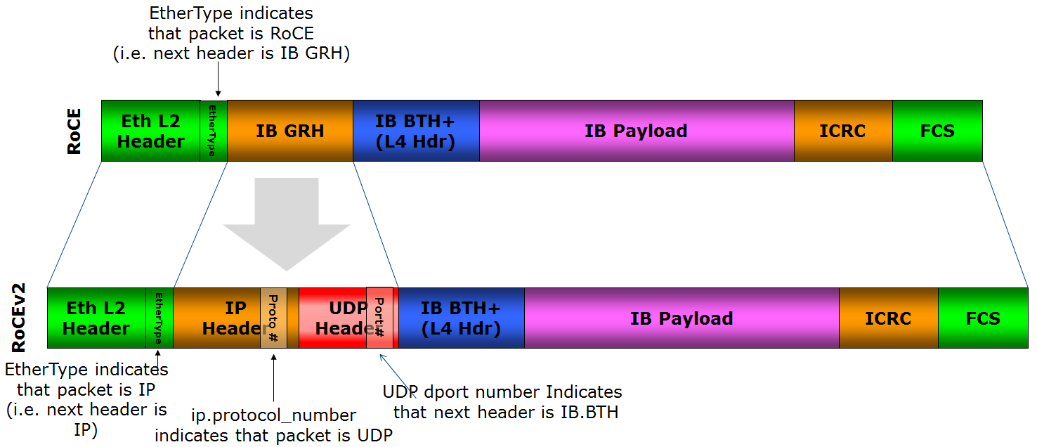
\includegraphics[width=\textwidth]{fig/RoCE_Header_format}
    \caption{RoCE v1 and RoCE v2 packet format}
    \label{fig:roce_header_format}
\end{figure*}

iWARP is an alternative to RoCE for bring RDMA to the Ethernet world. It implements RDMA on top of TCP stack, which is handled by the hardware directly.
Although it doesn't require additional configuration like PFC and run over a generic lossy network,
due to overhead of TCP stack, iWARP performance is much worse than RoCE and thus it hasn't been widely adopted.

\subsection{RDMA Security}

RDMA was originally designed for HPC clusters, where the entire cluster is isolated and trusted. It's thus safe to assume no eavesdropping or compromised switch.
However, recent adoptions of RDMA in datacenters changes the security model. In cloud environment, it's possible that malicious users might be able to either learn
side channel information by colocating their VM with victim VM, or even compromise other VMs. This demands that we prepare potential defense mechanism should such
attacks become realistic.

In the TCP world, SSL/TLS has been widely adopted for protecting the Web. \textcolor{red}{TBA}.

For RDMA, in a previous work, Security Enhancement in InfiniBand Archetecture~\cite{Lee:2005:SEI:1053727.1054449}, the paper achieves authenticity by embedding an authentication tag in the
header of an IBA packet. \textcolor{red}{TBA}
